\subsection{The Streaming Engine}

The SE is a coarse-grained fabric composed of compute tiles, which are interconnected with an SF, allowing data to traverse from one tile to another without queuing.
This SF allows many tiles to be pipelined together to produce a continuous data flow through SIMD arithmetic operations.
The tiles are also interconnected with an AF that allows synchronous domains of compute to be bridged by asynchronous operations.
These asynchronous operations include initiating synchronous domain operations, transferring data from one synchronous domain to another, accessing system memory (read and write), and performing branching and looping constructs.
Together, the SF nad AF allow the tiles to efficiently execute high level language constructs.

\begin{figure}
  \centering
  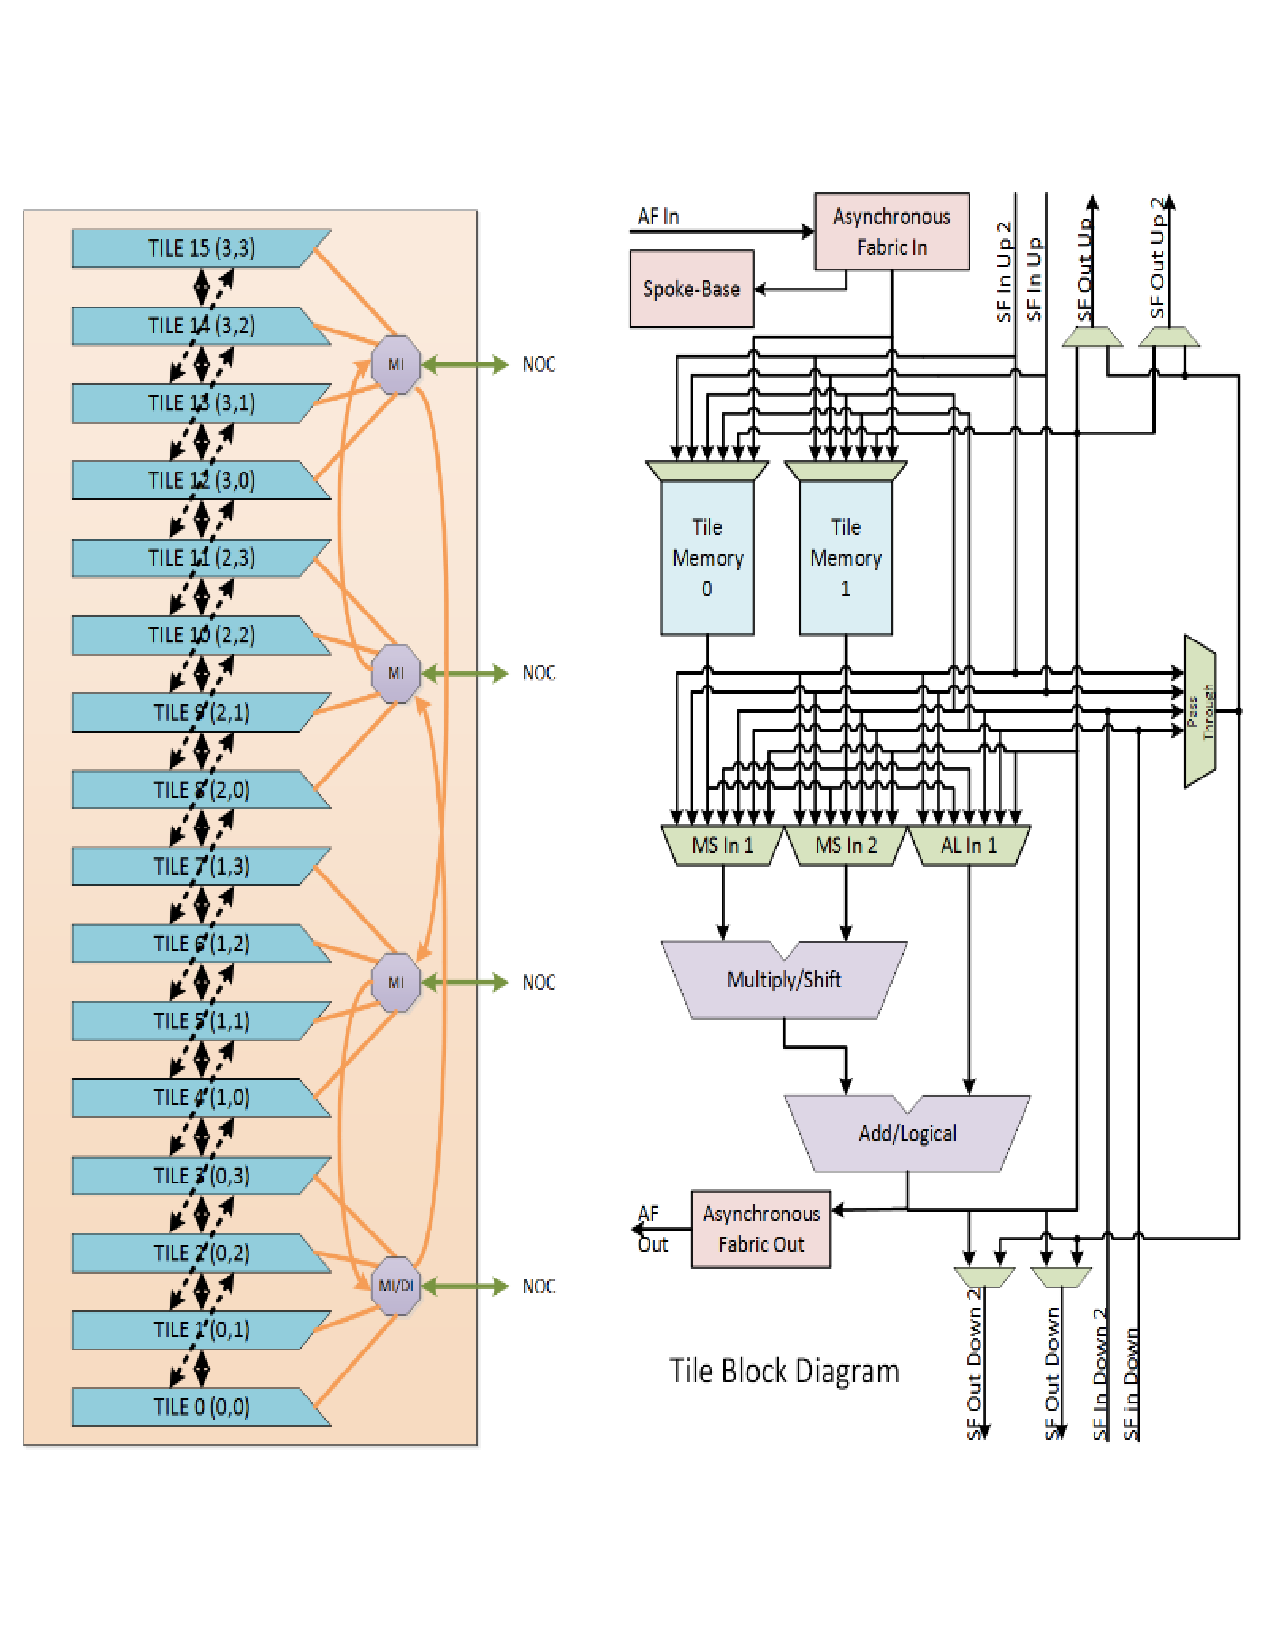
\includegraphics[width=\linewidth]{fig/se_device_tile.pdf}
  \caption{
    Diagram of the Streaming Engine.
  }
  \label{fig:se_diagram}
\end{figure}

As shown in the Fig. \ref{fig:se_diagram}, tiles are interconnected in a one by sixteen configuration.
The SF is used to connect a tile to another tile one hop above it, a tile two hops above it, a tile one hop below it and a tile two hops below it.
Information is transferred over the SF with a deterministic latency. 
Each tile acts independently, streaming data through internal memory and multiply-shift-ALU function units, to other tiles over the SF and AF.
The tiles use the AF to communicate between synchronous domains, send load and stores to memory through the MI, and receive commands from the host through the DI to initiate work on the SE.
Information is transferred over the AF with a non-deterministic latency.
The MI and DI communicate with memory and the Command Manager using the Network-On-Chip (NOC) interfaces.

In the computation graph to be mapped, each node represents an instruction that needs to be placed onto a SE tile. 
The edges of the graph represent the data dependencies of the instructions. 
The nodes also contain information about the variables that need to be present in tile memories during instruction execution. 
All data needed for the instruction must be present at the tile for the instruction to be executed. 
The tiles can pass data to their neighbors and each tile can be configured with a different number of initiation intervals (II). 
Each II can be allocated to run a single instruction during program execution. 
After one cycle, the tiles will move on to the next II, with execution returning to first II after the last. 
All tiles run the instruction in the same II in parallel. 
Thus, whenever possible, independent instructions should be mapped to different tiles and same II to exploit parallelism. 
The first operation of each disconnected component of the computation graph (one component representing a synchronous flow) 
needs to be placed on different tiles. 
The SE device configuration and its constraints are modeled in a simulation environment and the reward function. 
Violating a constraint or placing instructions sub-optimally leads to a reduced reward whereas placements that optimally 
reduce total execution time of the graph are rewarded. 
In Fig. \ref{fig:se_diagram}, the tiles connections that enables various possible instruction placements.